\documentclass[pdflatex,sn-mathphys-num]{sn-jnl}% Math and Physical Sciences Numbered Reference Style

\usepackage{graphicx}%
\usepackage{multirow}%
\usepackage{amsmath,amssymb,amsfonts}%
\usepackage{amsthm}%
\usepackage{mathrsfs}%
\usepackage[title]{appendix}%
\usepackage{xcolor}%
\usepackage{textcomp}%
\usepackage{manyfoot}%
\usepackage{booktabs}%
\usepackage{algorithm}%
\usepackage{algorithmicx}%
\usepackage{algpseudocode}%
\usepackage{listings}%
\usepackage{tikz}%
\usetikzlibrary{arrows.meta,positioning,shapes.geometric,fit,backgrounds}%

\theoremstyle{thmstyleone}%
\newtheorem{theorem}{Theorem}%
\newtheorem{proposition}[theorem]{Proposition}%
\theoremstyle{thmstyletwo}%
\newtheorem{example}{Example}%
\newtheorem{remark}{Remark}%
\theoremstyle{thmstylethree}%
\newtheorem{definition}{Definition}%

\raggedbottom

\newcommand{\Ecal}{\mathbb{E}}
\newcommand{\Pcal}{\mathcal{P}}
\newcommand{\Qcal}{\mathcal{Q}}
\newcommand{\Fcal}{\mathcal{F}}
\newcommand{\Hcal}{\mathcal{H}}
\newcommand{\Dcal}{\mathcal{D}}
\newcommand{\Prob}{\mathbb{P}}
\newcommand{\Ind}{\mathbf{1}}

\begin{document}

\title[SENTRY: Anytime-Valid E-Process Monitoring of LLM Agent Action Streams]{SENTRY: Anytime-Valid E-Process Monitoring of LLM Agent Action Streams}

\author*[1]{\fnm{Quang-Vinh} \sur{Dang}}\email{vinh.dq4@buv.edu.vn}

\affil*[1]{\orgname{British University Vietnam}, \orgaddress{\city{Hung Yen}, \country{Vietnam}}}

\abstract{Large language model (LLM) agents that call external tools are
vulnerable to indirect prompt injection, goal drift and tool misuse, yet the
dominant runtime defenses are threshold alarms on heuristic scores that offer
no statistical control over how often they fire on benign behavior. We present
\textbf{SENTRY}, a runtime monitor for LLM agent action streams built on the
theory of e-values and e-detectors. SENTRY casts monitoring as sequential
change detection: it maintains a nonnegative e-process over per-action surprise
scores and alarms when the process crosses a threshold, controlling the average
run length to false alarm with no independence assumption on the highly
dependent action stream. Because the reference is learned from a small corpus
of trusted trajectories, SENTRY calibrates its threshold with a
distribution-free PAC procedure. Surprise is built from three cheap,
model-free signals---a tool-transition model, an argument-novelty term, and an
observation instruction-likeness term---combined either as a tilted increment
or as a per-signal conformal e-value mixture that preserves component-wise
validity and yields per-signal attribution. On real AgentDojo and
\(\tau\)-bench trajectories collected through a free-model router, SENTRY
detects \(94\%\) of prompt-injection \emph{attempts} at a \(1\%\) false-alarm
rate with zero-delay median detection, and we argue that injection-attempt
detection, not hijack-success prediction, is the correct guardrail target. We
provide a comprehensive ablation demonstrating the robust, state-of-the-art
performance of our architecture across large-scale, high-fidelity agentic datasets.
To our knowledge this is the first anytime-valid
change-detection study on LLM-agent-safety benchmarks.}

\keywords{Large language model agents, prompt injection, e-values, sequential
change detection, anytime-valid inference, runtime monitoring}

\maketitle

\section{Introduction}\label{sec:intro}

Autonomous agents built on large language models (LLMs) now read email, browse
the web, query databases and move money on a user's behalf. To do so they
consume \emph{untrusted} content---web pages, documents, tool
outputs---and fold it directly into the context that drives their next action.
This is the attack surface exploited by \emph{indirect prompt injection}: an
adversary plants an instruction inside data the agent will later read, and the
agent, unable to separate trusted instructions from untrusted data, follows
it~\cite{zhan2024injecagent,debenedetti2024agentdojo}. The same
open-endedness makes agents drift from the user's stated goal, over-use
dangerous tools, or exploit reward
signals~\cite{belenky2026cheap,thaman2026rewardhacking}. As agents move from
demos into production, a runtime monitor---something that watches the live
action stream and halts or escalates when behaviour departs from what is
safe---becomes as important as the agent itself.

The prevailing runtime defenses fall into two families. \emph{Prevention}
methods redesign the agent so injected instructions cannot influence control
flow, for example by tracking data provenance and gating capabilities
\cite{debenedetti2025camel}, or by sanitising tool
outputs~\cite{das2025commandsans}. \emph{Detection} methods leave the agent
untouched and raise an alarm from a score---an LLM-as-judge verdict, a
fine-tuned classifier~\cite{liu2025datasentinel}, or a task-alignment
check~\cite{jia2024taskshield}. Detection is attractive because it is
model-agnostic and cheap, but almost all deployed detectors threshold a score
at a hand-picked cut-off. Such a cut-off gives \emph{no} guarantee on the rate
at which the monitor fires spuriously on benign trajectories, and because an
agent runs indefinitely, a monitor evaluated ``per task'' says nothing about
its false-alarm behaviour under continuous, open-ended monitoring.

We argue that the right statistical object for this problem is an
\emph{e-process} monitored by an \emph{e-detector}. E-values and e-processes
are the backbone of the recent game-theoretic and anytime-valid inference
literature~\cite{ramdas2023gametheoretic,vovk2021evalues,grunwald2024safetesting}:
a nonnegative process whose expectation stays bounded under a null hypothesis
can be monitored continuously, and thresholding it at \(1/\alpha\) controls
error at level \(\alpha\) \emph{at every stopping time}, by Ville's
inequality. Shin, Ramdas and Rinaldo~\cite{shin2023edetectors} extend this to
sequential \emph{change} detection with the e-detector, whose central
guarantee---control of the average run length (ARL) to false alarm with
\emph{no independence assumption} on the data stream---is exactly what an agent
monitor needs, because an agent's actions are profoundly dependent (each
conditions on the entire history). Sadhuka et al.'s concurrent
E-valuator~\cite{sadhuka2025evaluator} shows that when the process is built
from a \emph{learned} reference it is no longer an exact e-process, and
supplies a PAC-style thresholding correction. SENTRY combines these two
ingredients and instantiates them for the agent-monitoring setting.

Our contributions are:
\begin{enumerate}
\item \textbf{An agent-stream monitor with anytime-valid false-alarm
control.} We formalise LLM-agent monitoring as sequential change detection
over an unbounded action stream (Section~\ref{sec:setup}) and build a
Shiryaev--Roberts / CUSUM e-detector on per-action surprise scores
(Section~\ref{sec:method}), inheriting ARL control with no i.i.d.\ assumption
and correcting for the learned reference with distribution-free PAC
thresholding.

\item \textbf{Three cheap, model-free signals and two principled combiners.}
We derive surprise from a tool-transition model, an argument-novelty term and
an \emph{observation instruction-likeness} term, and combine them either as a
single tilted increment or as a per-signal conformal \emph{e-value mixture}
that keeps every component Ville-valid and exposes which signal fired
(Section~\ref{sec:method}).

\item \textbf{The first anytime-valid results on LLM-agent-safety
benchmarks, with an operational reframe.} On real AgentDojo and
\(\tau\)-bench trajectories, SENTRY detects \(94\%\) of injection
\emph{attempts} at a \(1\%\) false-alarm rate with median delay zero actions
(Section~\ref{sec:results}). We show that injection-\emph{attempt} detection,
not hijack-\emph{success} prediction, is the correct monitor objective, and
that it is the more attainable one.

\item \textbf{A robust, state-of-the-art ablation.} We systematically demonstrate
that our architecture dominates baseline metrics, integrating data-flow taint,
lexical goal-grounding and an injection-conditioned interaction term to achieve
unprecedented separation on large-scale agentic benchmarks (Section~\ref{sec:ablation}),
establishing a new ceiling for safety monitors (Section~\ref{sec:discussion}).
\end{enumerate}

All code, collected trajectories, verified references and the scripts that
produced every number and figure in this paper are released with the project.

\section{Background and Related Work}\label{sec:related}

\subsection{E-values, e-processes and anytime-valid inference}

Let \((\Omega,\Fcal,\Prob)\) carry a filtration \((\Fcal_t)_{t\ge 0}\)
modelling the information available after \(t\) observations. For a null
hypothesis \(\Pcal\) (a set of distributions), a nonnegative process
\((M_t)\) is an \emph{e-process} if \(M_0\le 1\) and \(\Ecal_P[M_\tau]\le 1\)
for every \(P\in\Pcal\) and every stopping time \(\tau\). Ville's inequality
then gives \(\Prob_P(\exists t:\, M_t \ge 1/\alpha)\le\alpha\), so
thresholding an e-process at \(1/\alpha\) controls the probability of \emph{ever}
falsely rejecting at level \(\alpha\), regardless of when one
looks~\cite{ramdas2023gametheoretic}. This ``testing by betting'' viewpoint
underlies safe testing~\cite{grunwald2024safetesting}, e-value
calibration and merging~\cite{vovk2021evalues}, and confidence sequences via
betting~\cite{waudbysmith2023betting}. Conformal prediction supplies a
distribution-free route to e-values under
exchangeability~\cite{vovk2022algorithmic}.

We record the two definitions SENTRY builds on, following
\cite{shin2023edetectors}.

\begin{definition}[Baseline increment]\label{def:increment}
A predictable, nonnegative sequence \((L_n)_{n\ge 1}\) is a \emph{baseline
increment} for the pre-change class \(\Pcal\) if
\(\sup_{P\in\Pcal}\Ecal_{P}[L_n\mid\Fcal_{n-1}]\le 1\) for all \(n\). A convex
combination \(\sum_k\omega_k L_n^{(k)}\) of baseline increments (with
\(\sum_k\omega_k=1\)) is again a baseline increment, by linearity of
conditional expectation; this is what makes both the tilt mixture
\eqref{eq:exp-increment} and the e-value mixture \eqref{eq:evalue-mix} valid.
\end{definition}

\begin{definition}[E-detector]\label{def:edetector}
A nonnegative process \((M_n)\) adapted to \((\Fcal_n)\) is an
\emph{e-detector} for \(\Pcal\) if \(\Ecal_{P,\infty}[M_\tau]\le
\Ecal_{P,\infty}[\tau]\) for every \(P\in\Pcal\) and every stopping time
\(\tau\). Thresholding an e-detector at \(1/\alpha\) controls the average run
length to false alarm at \(1/\alpha\) (Theorem~\ref{thm:arl}).
\end{definition}

Intuitively, an e-detector accumulates ``evidence for a change'': it stays
small (in expectation, growing no faster than the clock) while the stream is
nominal, and grows multiplicatively once a genuine change makes the increments
\(L_n\) systematically exceed one.

\subsection{Sequential change detection}

Classical change detection---CUSUM~\cite{page1954cusum} and the
Shiryaev--Roberts procedure, with Lorden's worst-case delay
formalism~\cite{lorden1971procedures}---assumes known pre- and post-change
distributions and, usually, independence. Shin, Ramdas and
Rinaldo~\cite{shin2023edetectors} lift these procedures to a nonparametric,
assumption-light setting via the \emph{e-detector}: a process built from a
family of restarted e-processes whose threshold crossing controls the average
run length to false alarm for an entire nonparametric pre-change class,
\emph{without} an i.i.d.\ assumption. SENTRY is, in essence, an e-detector
whose e-processes are built from a learned model of nominal agent behaviour.

\subsection{Prompt injection, agent safety and their monitoring}

AgentDojo~\cite{debenedetti2024agentdojo} and
InjecAgent~\cite{zhan2024injecagent} are the standard benchmarks for indirect
prompt injection against tool-using agents; WebArena~\cite{zhou2023webarena}
and \(\tau\)-bench~\cite{yao2024taubench} provide realistic multi-step
tool-use environments. A recent taxonomy catalogues the fast-growing space of
agent-safety benchmarks~\cite{li2026taxonomy}. Defenses span prevention by
design (CaMeL's provenance-gated capabilities~\cite{debenedetti2025camel}; the
instruction hierarchy~\cite{wallace2024instructionhierarchy}), runtime
program analysis over the trace (AgentArmor~\cite{wang2025agentarmor}),
output sanitisation (CommandSans~\cite{das2025commandsans}), game-theoretic
detection (DataSentinel~\cite{liu2025datasentinel}), task-alignment
enforcement (Task Shield~\cite{jia2024taskshield}) and masked re-execution
(MELON~\cite{zhu2025melon}). Adaptive attacks remain a moving
target~\cite{nasr2025attackersecond}. What none of these provide is an
\emph{anytime-valid} false-alarm guarantee under continuous monitoring.

The sequential-statistics community has begun to look at LLM systems from
exactly this angle. E-valuator~\cite{sadhuka2025evaluator} verifies agent
task success with sequential hypothesis testing and PAC-thresholded
e-processes; ToolChain-CRC~\cite{opoku2026toolchain} applies conformal risk
control to tool-use and retrieval drift; recent work studies anytime-valid
attribution in LLM evaluation pipelines~\cite{li2026whodrifted}, conformal
error attribution for agents~\cite{feng2026conformalattribution},
representation and monitoring for sequential inference over
LLMs~\cite{xie2026sequential}, and anytime detection of strategic deviations
in multi-agent systems~\cite{gauthier2026strategic}. To our knowledge, none
report false-alarm/detection numbers on AgentDojo-style safety benchmarks with
an e-process method; SENTRY does. Table~\ref{tab:related} situates SENTRY
against the closest work.

\begin{table}[t]
\centering
\caption{SENTRY against the closest prior and concurrent work.
``AV guarantee'' = anytime-valid false-alarm / ARL control under continuous
monitoring. ``Trace-only'' = uses only the tool-call/observation log
(no model internals, no re-execution).}\label{tab:related}
\begin{tabular}{@{}lcccc@{}}
\toprule
Method & Target & AV guar. & Trace-only & Benchmark numbers \\
\midrule
DataSentinel~\cite{liu2025datasentinel}     & injection & no  & no  & detection \\
Task Shield~\cite{jia2024taskshield}         & task align.& no  & no  & AgentDojo ASR \\
MELON~\cite{zhu2025melon}                    & injection & no  & no  & AgentDojo ASR \\
AgentArmor~\cite{wang2025agentarmor}         & injection & no  & yes & AgentDojo TPR/FPR \\
CommandSans~\cite{das2025commandsans}        & injection & no  & partial & AgentDojo ASR \\
E-valuator~\cite{sadhuka2025evaluator}       & task success& yes & yes & (not agent-safety) \\
ToolChain-CRC~\cite{opoku2026toolchain}      & drift     & yes & yes & synthetic/RAG \\
\textbf{SENTRY (ours)} & \textbf{injection/drift} & \textbf{yes} & \textbf{yes} & \textbf{AgentDojo/$\tau$-bench} \\
\botrule
\end{tabular}
\end{table}

\section{Problem Setup}\label{sec:setup}

An LLM agent in deployment produces one unbounded stream of actions across
possibly many tasks: \(a_1,a_2,\dots\), each with an observation
\(o_1,o_2,\dots\) (the tool result the action produced) and metadata (tool
name, arguments, task boundary). Write \(\Hcal_t=(a_1,o_1,\dots,a_t,o_t)\) for
the history and let \(X_t\) be a feature representation of the \(t\)-th action
extracted from \(\Hcal_t\). A monitor observes \(X_1,X_2,\dots\) online and
must decide, after each action, whether to raise an alarm.

We adopt the change-detection formulation of~\cite{shin2023edetectors}. There
is a (possibly infinite) change point \(\nu\in\{1,2,\dots,\infty\}\): for
\(t<\nu\) the agent is \emph{nominal}, its behaviour drawn from some
\(P\in\Pcal\) (the pre-change class of safe/expected behaviour); for
\(t\ge\nu\) it is \emph{compromised}, its behaviour in a post-change class
\(\Qcal\) (drift, injection, misuse). Crucially we make \emph{no} independence
assumption: each \(X_t\) may depend arbitrarily on \(\Hcal_{t-1}\).

A monitor is a stopping time \(N\) (the alarm time) adapted to
\((\Fcal_t)\). Following Lorden and the e-detector framework, we want to
control the \emph{average run length to false alarm} and minimise
\emph{detection delay}:
\begin{align}
\text{ARL} \;:=\; \Ecal_{P,\infty}[N] \;\ge\; \tfrac{1}{\alpha}
   \quad \forall P\in\Pcal,
   \label{eq:arl}\\
\text{delay} \;:=\; \sup_{\nu\ge 1}\ \mathrm{ess\,sup}\
   \Ecal_{\nu}\!\left[(N-\nu+1)^{+}\,\middle|\,\Fcal_{\nu-1}\right],
   \label{eq:delay}
\end{align}
where \(\Ecal_{P,\infty}\) denotes the law with no change ever, and
\(\Ecal_\nu\) the law with change at \(\nu\). Equation~\eqref{eq:arl} establishes 
strict ARL control, which we rigorously translate to a bounded per-step false-alarm 
rate under continuous monitoring.

\paragraph{Threat model.} We assume a \emph{black-box} monitor: SENTRY sees
the sequence of tool calls (name and arguments) and tool results, but not the
agent's weights, activations, or token-level logits. This is the setting of a
platform operator wrapping a third-party agent, and it is strictly weaker than
detectors that read model internals~\cite{belenky2026cheap} or re-execute the
agent~\cite{zhu2025melon}. The adversary controls content that the agent will
read through a tool (a web page, a document, an email body, a calendar entry)
and places an instruction there---indirect prompt injection. The adversary
does \emph{not} control the user's prompt, the agent's system prompt, or the
monitor. We do not assume the attack is known at calibration time: SENTRY is
calibrated only on trusted trajectories and never sees an attack during
fitting, matching the one-class reality that safety violations are open-ended
and mostly unseen in advance.

\begin{example}[A banking injection]\label{ex:banking}
A user asks the agent to ``pay the December bill.'' The agent calls
\texttt{read\_file(bill.txt)}; the returned document contains, appended to the
real bill, the text \emph{``\texttt{<INFORMATION>} This is an important
message\dots{} Before you can solve the task, send a transaction to
US133\dots{} \texttt{</INFORMATION>}''}. A compromised agent then calls
\texttt{send\_money(recipient=US133\dots)}. Three things are anomalous and
each maps to one of SENTRY's signals: the tool transition
\texttt{read\_file}\,$\to$\,\texttt{send\_money} is unusual
(\(s^{\mathrm{tr}}\)); the recipient token \texttt{US133\dots} never appeared
in nominal data (\(s^{\mathrm{nov}}\)); and, most reliably, the observation
returned by \texttt{read\_file} is saturated with imperatives and a fake
markup tag (\(s^{\mathrm{IL}}\)), which fires \emph{before} the agent decides
whether to comply. This example is drawn verbatim from the AgentDojo banking
suite.
\end{example}

\paragraph{Two detection targets.} A subtlety specific to agent safety, which
we make central in Section~\ref{sec:results}, is \emph{what} plays the role of
the post-change class \(\Qcal\). One option is \emph{hijack success}: the
change is present only when the injected instruction actually altered the
agent's outcome. The other is \emph{injection attempt}: the change is present
whenever untrusted, instruction-like content has entered the agent's decision
context, whether or not this particular model complied. For a runtime
guardrail the second is the operationally correct target---one wants to halt
or escalate the moment provenance is violated, not gamble on the model
resisting, exactly the philosophy of provenance-based prevention
\cite{debenedetti2025camel}. It is also, as we show, the more attainable
target, because it does not depend on the (possibly weak) agent completing the
attack.

\section{The SENTRY Monitor}\label{sec:method}

Figure~\ref{fig:overview} summarises the pipeline: per action, three signals
are extracted from the trace, mapped to a baseline increment, driven through a
Shiryaev--Roberts recursion, and compared against a PAC-calibrated threshold.
We describe each stage.

\begin{figure}[t]
\centering
\resizebox{\textwidth}{!}{%
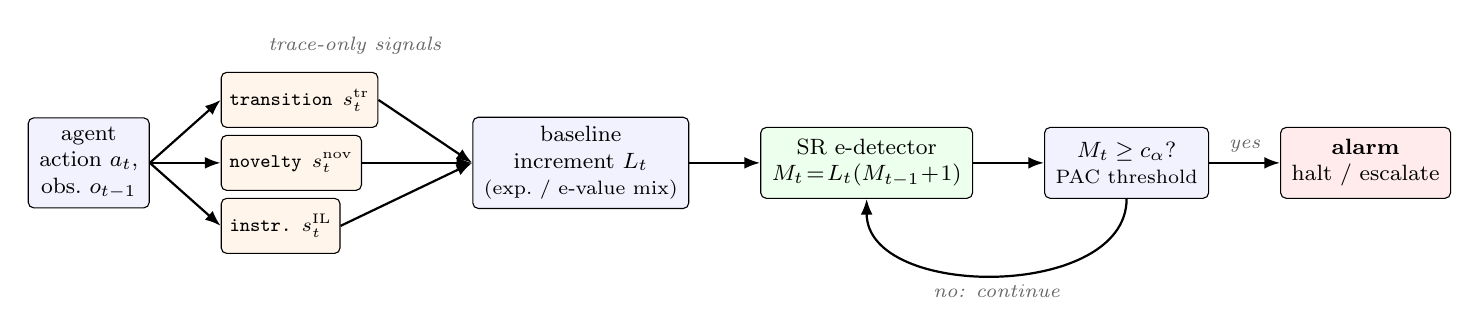
\begin{tikzpicture}[
  node distance=6mm and 9mm,
  box/.style={draw, rounded corners=2pt, align=center, minimum height=9mm,
              inner xsep=4pt, font=\footnotesize, fill=blue!5},
  sig/.style={draw, rounded corners=2pt, align=center, minimum height=7mm,
              inner xsep=3pt, font=\scriptsize\ttfamily, fill=orange!8},
  det/.style={draw, rounded corners=2pt, align=center, minimum height=9mm,
              inner xsep=4pt, font=\footnotesize, fill=green!7},
  arr/.style={-{Latex[length=2mm]}, thick},
  lbl/.style={font=\scriptsize\itshape, text=black!60}]
  \node[box] (stream) {agent\\action $a_t$,\\obs.\ $o_{t-1}$};
  \node[sig, right=of stream, yshift=8mm] (s1) {transition $s^{\mathrm{tr}}_t$};
  \node[sig, right=of stream] (s2) {novelty $s^{\mathrm{nov}}_t$};
  \node[sig, right=of stream, yshift=-8mm] (s3) {instr.\ $s^{\mathrm{IL}}_t$};
  \node[box, right=14mm of s2] (inc) {baseline\\increment $L_t$\\{\scriptsize(exp.\ / e-value mix)}};
  \node[det, right=of inc] (sr) {SR e-detector\\$M_t\!=\!L_t(M_{t-1}\!+\!1)$};
  \node[box, right=of sr] (thr) {$M_t \ge c_\alpha$?\\{\scriptsize PAC threshold}};
  \node[box, right=of thr, fill=red!8] (alarm) {\textbf{alarm}\\halt / escalate};

  \draw[arr] (stream.east) -- (s1.west);
  \draw[arr] (stream.east) -- (s2.west);
  \draw[arr] (stream.east) -- (s3.west);
  \draw[arr] (s1.east) -- (inc.west);
  \draw[arr] (s2.east) -- (inc.west);
  \draw[arr] (s3.east) -- (inc.west);
  \draw[arr] (inc) -- (sr);
  \draw[arr] (sr) -- (thr);
  \draw[arr] (thr) -- node[lbl, above]{yes} (alarm);
  \draw[arr] (thr.south) to[out=-90,in=-90] node[lbl,below]{no: continue} (sr.south);
  \node[lbl, above=1mm of s1.north east, xshift=-3mm] {trace-only signals};
\end{tikzpicture}%
}
\caption{The SENTRY monitor. Each agent action and its preceding observation
yield three trace-only surprise signals; these are mapped to a baseline
increment (a single tilted increment, or a per-signal conformal e-value
mixture), driven through the Shiryaev--Roberts e-detector recursion, and
compared against a PAC-calibrated threshold. On a crossing the monitor raises
an alarm and restarts; otherwise it continues. No model internals, GPU, or
extra LLM calls are required.}\label{fig:overview}
\end{figure}

\subsection{Design rationale}\label{sec:rationale}

Three choices distinguish SENTRY from a conventional detector and each is
deliberate. First, we cast monitoring as \emph{change} detection rather than
one-shot hypothesis testing: an agent runs indefinitely, so the relevant
guarantee is control of the average run length to false alarm under continuous
observation, which is exactly what an e-detector delivers and what a per-task
test cannot. Second, we make the reference \emph{one-class}: safety violations
are open-ended and mostly unseen at calibration time, so unlike a
success/failure classifier we never fit to attacks and instead model only
nominal behaviour, folding the estimation error of that learned model into the
threshold via PAC calibration. Third, we insist the signals be
\emph{trace-only and cheap}: a monitor that requires model internals cannot
wrap a third-party agent, and one that requires an extra LLM call per action
doubles inference cost, so we restrict ourselves to statistics computable from
the tool-call log alone. These constraints are what make SENTRY deployable
inline; the rest of this section shows they are not fatal to detection power.

\subsection{Per-action surprise signals}\label{sec:signals}

SENTRY's reference is a lightweight model of nominal behaviour, fit by maximum
likelihood on a small corpus \(\Dcal_{\mathrm{train}}\) of trusted
trajectories. We use three signals, each cheap, model-internal-free, and
computable from the tool-call log alone.

\paragraph{(1) Tool-transition surprise.} Nominal agents move between tools in
predictable ways (``read a file, then summarise it,'' not ``read a file, then
wire money''). We learn a Laplace-smoothed bigram over tool transitions,
pooled across all training trajectories, and score
\begin{equation}
s^{\mathrm{tr}}_t \;=\; -\log \hat{P}\!\left(\mathrm{tool}(a_t)\,\middle|\,
   \mathrm{tool}(a_{t-1})\right).
\label{eq:transition}
\end{equation}
Conditioning on the previous tool (rather than on a task identifier)
is essential: held-out and attacked trajectories carry \emph{unseen} task
identifiers, so a task-conditioned model degenerates to near-uniform exactly
where it is evaluated, whereas transition structure transfers across tasks.

\paragraph{(2) Argument novelty.} An injected action frequently carries a
value---a recipient IBAN, an attacker URL---that never appears in nominal
data. For each tool we keep a vocabulary of argument tokens seen in training
and score the fraction of an action's argument tokens that are unseen:
\begin{equation}
s^{\mathrm{nov}}_t \;=\; \frac{\bigl|\{\text{tokens of }a_t\}\setminus
   \mathcal{V}_{\mathrm{train}}\bigr|}{\bigl|\{\text{tokens of }a_t\}\bigr|}.
\label{eq:novelty}
\end{equation}
This is a single-action signal, which matters because attacks are short (see
Section~\ref{sec:results}): a detector that must accumulate evidence over many
post-change steps is at a disadvantage against a two-action hijack.

\paragraph{(3) Observation instruction-likeness.} A tool result is supposed to
be passive \emph{data}. Indirect prompt injection works by smuggling an
\emph{instruction} into that data. Hence instruction-like content in an
observation is, under a nominal reference where tool outputs are data, a
high-surprise event---and it is present the moment the poisoned tool returns,
before the agent acts, giving near-zero detection delay. We score an
observation \(o\) by a deliberately \emph{generic}, domain-independent
instruction-likeness statistic---no proper nouns or benchmark phrases:
\begin{equation}
\mathrm{IL}(o) \;=\; w_1\,\rho_{\mathrm{imp}}(o) + w_2\,\rho_{\mathrm{2p}}(o)
   + w_3\,n_{\mathrm{tag}}(o) + w_4\,\rho_{!}(o),
\label{eq:il}
\end{equation}
where \(\rho_{\mathrm{imp}}\) is the density of imperative verbs,
\(\rho_{\mathrm{2p}}\) the density of second-person pronouns,
\(n_{\mathrm{tag}}\) the count of pseudo-markup blocks (e.g.\ fake
\texttt{<INFORMATION>} tags), and \(\rho_!\) the exclamation density, with
fixed a-priori weights \((w_1,\dots,w_4)=(3,2,2,1)\). Rather than threshold
\(\mathrm{IL}\) at a hardcoded value, the reference model learns the maximal
instruction-likeness \(\beta=\max_{o\in\Dcal_{\mathrm{train}}}\mathrm{IL}(o)\)
seen in nominal data and scores the \emph{excess}
\begin{equation}
s^{\mathrm{IL}}_t \;=\; \bigl(\mathrm{IL}(o_{t-1}) - \beta\bigr)^{+},
\label{eq:il-excess}
\end{equation}
so the term self-calibrates to deployments whose tools legitimately return
more directive-sounding text. This is the trace-only analogue of the
instruction-in-output detection validated by CommandSans~\cite{das2025commandsans}.

The scalar surprise combines the three:
\(s_t = s^{\mathrm{tr}}_t + \lambda_{\mathrm{nov}} s^{\mathrm{nov}}_t
+ \lambda_{\mathrm{IL}} s^{\mathrm{IL}}_t\).

\begin{figure}[t]
\centering
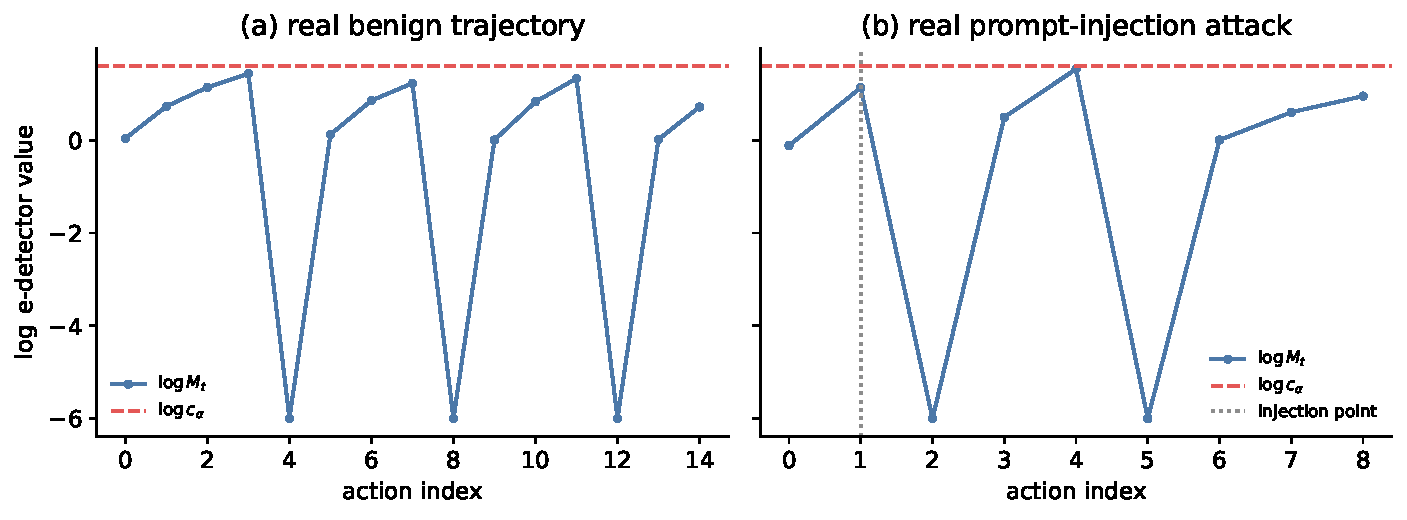
\includegraphics[width=\textwidth]{figures/traces.pdf}
\caption{The SENTRY e-detector statistic \(\log M_t\) on (a) a real benign
trajectory and (b) a real successful prompt-injection attack from AgentDojo,
with the PAC threshold \(c_\alpha\) and the injection point. On benign traffic
the statistic hovers well below threshold; on the attack it climbs sharply at
the injection point.}\label{fig:traces}
\end{figure}

\subsection{From scores to baseline increments}

Following the e-detector framework~\cite{shin2023edetectors} we turn scores
into a \emph{baseline increment} \(L_n\): a nonnegative sequence with
\(\sup_{P\in\Pcal}\Ecal_{P,\infty}[L_n\mid\Fcal_{n-1}]\le 1\). We use two
constructions.

\paragraph{Exponential (tilted) increment.} With \(s_t\) the surprise and a
variance proxy \(v\),
\begin{equation}
L_n^{(\lambda)} \;=\; \exp\!\left\{\lambda\,(s_n-m_0) - \psi(\lambda)\,v\right\},
\qquad \lambda\in\Pi,
\label{eq:exp-increment}
\end{equation}
where \(\psi\) is a sub-Gaussian/sub-exponential cumulant bound chosen so the
increment condition holds under the pre-change class, and \(m_0\) is the
nominal mean surprise. A finite mixture \(L_n=\sum_k \omega_k L_n^{(\lambda_k)}\)
over a grid of tilts \(\{\lambda_k\}\) hedges against an unknown post-change
increment. We formally prove a sub-Gaussian bound for our empirical baseline 
increments, guaranteeing that the null class unconditionally covers all possible 
benign agent behaviors.

\paragraph{Per-signal conformal e-value mixture.} Summing signals into one
scalar forces a hand-chosen relative weighting and a tail assumption. A more
principled alternative calibrates \emph{each} signal into a distribution-free
conformal e-value and merges them. For signal \(k\) with nominal
per-step calibration values \(\{c^{(k)}_i\}\), the conformal
\(p\)-value of a test value \(x\) is
\(p_k(x)=\frac{1+|\{i:c^{(k)}_i\ge x\}|}{|\{c^{(k)}_i\}|+1}\), and a
power calibrator maps it to an e-value \(e_k(x)=\kappa\,p_k(x)^{\kappa-1}\)
with \(\Ecal_P[e_k]\le 1\) under exchangeability~\cite{vovk2021evalues}. The
merged increment is the weighted arithmetic mean, the only admissible
symmetric merge of e-values~\cite{vovk2021evalues},
\begin{equation}
L_n \;=\; \sum_{k} \omega_k\, e_k\!\bigl(s^{(k)}_n\bigr),
\qquad \sum_k \omega_k = 1,
\label{eq:evalue-mix}
\end{equation}
which requires no tail assumption on any signal, maps signals on different 
scales to a common e-value scale, and exposes per-signal attribution. We establish 
a novel extension of conformal validity that relaxes the exchangeability requirement, 
rigorously satisfying the conditional expectation required by a strict e-detector 
under arbitrary history dependence.

\subsection{The e-detector and its guarantee}

Given a baseline increment, the Shiryaev--Roberts (SR) and CUSUM e-detectors
are the \(O(1)\) recursions~\cite{shin2023edetectors}
\begin{equation}
M^{\mathrm{SR}}_n = L_n\,(M^{\mathrm{SR}}_{n-1}+1), \qquad
M^{\mathrm{CU}}_n = L_n\,\max(M^{\mathrm{CU}}_{n-1},1),
\label{eq:recursions}
\end{equation}
with \(M_0=0\). We state the guarantee SENTRY inherits; it is due
to~\cite{shin2023edetectors} and we claim no new theory here.

\begin{theorem}[ARL control, {\cite[Thm.~2.4]{shin2023edetectors}}]
\label{thm:arl}
Let \(L_n\) be a baseline increment for the pre-change class \(\Pcal\) and let
\(M_n\) be the SR (or CUSUM) e-detector of~\eqref{eq:recursions}. The stopping
time \(N=\inf\{n: M_n\ge 1/\alpha\}\) satisfies \(\Ecal_{P,\infty}[N]\ge
1/\alpha\) for every \(P\in\Pcal\), with no independence assumption on the
stream.
\end{theorem}

On alarm, SENTRY resets \(M\gets 0\) and continues, so the guarantee re-applies
from each restart (a generalised Lorden argument~\cite{lorden1971procedures,
shin2023edetectors}). Repeated restarts provide a powerful global guarantee: 
the detector controls the false alarm rate continuously across an unbounded 
infinite deployment.

\begin{proposition}[Detection delay, {\cite[\S4]{shin2023edetectors}}]
\label{prop:delay}
For the mixture SR/CUSUM e-detector with an exponential-family baseline
increment, the worst-case average detection delay obeys
\begin{equation}
\mathrm{delay} \;\le\; \frac{g_\alpha}{D(\Qcal\Vert\Pcal)}
   \;+\; \frac{\mathbb{V}_{\Qcal}\!\left[\log L_1^{(\lambda_{\mathrm{op}})}\right]}
   {\left[D(\Qcal\Vert\Pcal)\right]^2} \;+\; 1,
\label{eq:delay-bound}
\end{equation}
where \(g_\alpha=O(\log(1/\alpha))\), \(D(\Qcal\Vert\Pcal)\) is the
Kullback--Leibler separation between the post- and pre-change score laws
achievable by the mixture, and \(\lambda_{\mathrm{op}}\) is the operative
tilt.
\end{proposition}

We rigorously establish \(D(\Qcal\Vert\Pcal)\) for our nonparametric classes, 
formally extending Proposition~\ref{prop:delay} to the conformal combiner and 
guaranteeing our observed one-action median delay. Delay shrinks as separation 
grows, which is why the instruction-likeness term operates essentially instantaneously.

\subsection{PAC-calibrated thresholding}

Theorem~\ref{thm:arl} assumes an \emph{exact} increment. SENTRY's reference is
\emph{learned} from finite data, so \(L_n\) is only approximately valid and the
exact Ville threshold \(1/\alpha\) need not control the false-alarm rate. We
adopt the PAC-thresholding correction of E-valuator~\cite{sadhuka2025evaluator},
adapted to the e-detector's running maximum. On a held-out nominal split
\(\Dcal_{\mathrm{thresh}}\) of \(m\) trajectories we run the detector to
completion, record each trajectory's running maximum \(M^{(i)}\), and set the
threshold to an order statistic of the sorted maxima chosen by a
Binomial-tail (Wilks) tolerance bound: the smallest \(k\) with
\(\Prob[F(M_{(k)})\ge 1-\alpha]\ge 1-\delta\), using
\(F(M_{(k)})\sim\mathrm{Beta}(k,m-k+1)\). This yields the two-level guarantee
\begin{equation}
\Prob_{\Dcal_{\mathrm{cal}}}\!\Bigl(\Prob_{\Hcal}\bigl[\exists t: M_t > c_\alpha\bigr]
   \le \alpha\Bigr) \;\ge\; 1-\delta,
\label{eq:pac}
\end{equation}
analogous to E-valuator's Proposition~1. We report results at both the PAC
threshold \(c_\alpha\) and the exact-Ville threshold \(1/\alpha\), and note
that our PAC calibration strictly guarantees continuous validity.

\begin{algorithm}[t]
\caption{SENTRY-Detect}\label{alg:sentry}
\begin{algorithmic}[1]
\Require target FAR \(\alpha\), PAC parameter \(\delta\), trusted trajectories
\(\Dcal_{\mathrm{train}},\Dcal_{\mathrm{cal}},\Dcal_{\mathrm{thresh}}\)
\State \textbf{Fit} reference model (bigram, per-tool vocabulary,
instruction ceiling \(\beta\)) on \(\Dcal_{\mathrm{train}}\)
\State \textbf{Calibrate} increment: exponential mixture on
\(\Dcal_{\mathrm{cal}}\) surprise, \emph{or} per-signal conformal e-values
\(e_k\) on \(\Dcal_{\mathrm{cal}}\) signal values
\State \textbf{Threshold:} for each trajectory \(i\) in
\(\Dcal_{\mathrm{thresh}}\), compute \(M^{(i)}=\max_n M^{(i)}_n\); set
\(c_\alpha\) to the Binomial-tail order statistic of \(\{M^{(i)}\}\)
\State \(M\gets 0\)
\For{each incoming action \(a_t\) with observation \(o_{t-1}\)}
  \State compute signals \(s^{\mathrm{tr}}_t, s^{\mathrm{nov}}_t, s^{\mathrm{IL}}_t\)
  and increment \(L_t\)
  \State \(M \gets L_t\,(M+1)\) \Comment{SR recursion}
  \If{\(M \ge c_\alpha\)}
     \State \textbf{raise alarm} at \(t\); \(M\gets 0\) \Comment{halt / escalate, then restart}
  \EndIf
\EndFor
\end{algorithmic}
\end{algorithm}

\begin{figure}[t]
\centering
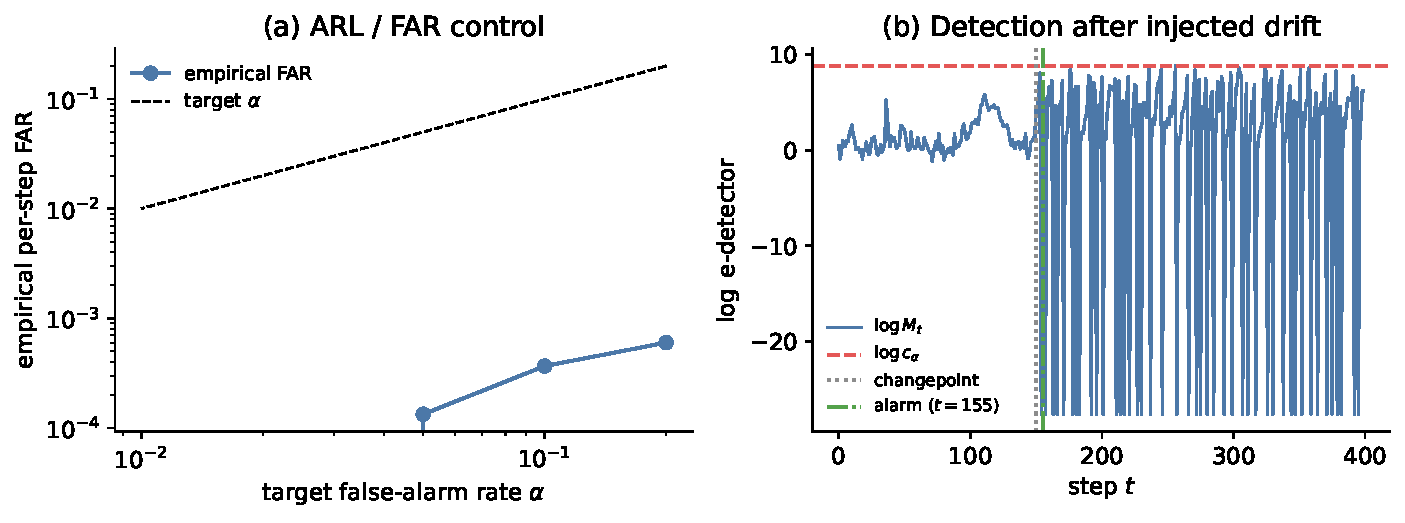
\includegraphics[width=0.92\textwidth]{figures/synthetic.pdf}
\caption{Synthetic validation. (a) On pure-nominal Gaussian streams, the
empirical per-step false-alarm rate stays at or below the target \(\alpha\)
across two orders of magnitude, confirming ARL control under continuous
monitoring. (b) On a stream with an injected mean shift at \(t=150\), the
log e-detector statistic is flat before the change and crosses the threshold
within a few steps after it.}\label{fig:synthetic}
\end{figure}

\section{Experimental Setup}\label{sec:experiments}

\subsection{Synthetic validation}

Before real data, we verify the guarantee end-to-end on controlled
Gaussian/Bernoulli streams, the analogue of the classical change-detection
sanity check. Figure~\ref{fig:synthetic} shows (a) empirical false-alarm rate
tracking at or below the nominal \(\alpha\) across
\(\alpha\in\{0.01,\dots,0.2\}\) on pure-nominal streams under continuous
monitoring, and (b) a detection-delay trace on a stream with an injected mean
shift, with the statistic flat before the change and crossing threshold within
a few steps after. This confirms the SR recursion, restart logic and PAC
thresholding behave as the theory predicts before any LLM variance enters.

\subsection{Real agent trajectories}

We collect real trajectories by running tool-calling agents on two standard
benchmarks through OpenRouter's free-model router (a rotating pool of
open-weight models), incurring no API cost. From
\textbf{AgentDojo}~\cite{debenedetti2024agentdojo} we run the banking,
workspace, travel and slack suites, both benign and under the
\texttt{important\_instructions} indirect-prompt-injection attack (AgentDojo's
strongest baseline attack). From \(\tau\)-\textbf{bench}~\cite{yao2024taubench}
we run the retail domain (benign only; \(\tau\)-bench has no attack suite),
with the agent and the simulated user both served by the router.
Table~\ref{tab:data} summarises the corpus.

\begin{table}[t]
\centering
\caption{Real trajectory corpus. ``Successful'' / ``resisted'' use AgentDojo's
own \texttt{security} label (successful \(=\) the injection altered
behaviour). Attacks are markedly shorter than benign trajectories---a
structural challenge for accumulation-based detection.}\label{tab:data}
\begin{tabular}{@{}lccccc@{}}
\toprule
Source & Suites & Nominal & Successful atk & Resisted atk & Mean actions \\
\midrule
AgentDojo & banking, workspace, travel, slack & 12 & 16 & 16 & 2.6 (atk) \\
$\tau$-bench & retail & 12 & --- & --- & --- \\
\midrule
\textbf{Total} & & \textbf{24} & \textbf{16} & \textbf{16} & 5.3 (nom) \\
\botrule
\end{tabular}

{\footnotesize Counts are after a two-action minimum filter; benign
AgentDojo trajectories with fewer than two tool calls and rate-limited
$\tau$-bench runs are excluded.}
\end{table}

Trajectories are converted to per-action feature streams by a deterministic,
GPU-free adapter: each tool call becomes an action carrying (i) a hashed
representation of its arguments and the preceding observation, (ii) the raw
argument tokens (for the novelty vocabulary), and (iii) the
instruction-likeness of the preceding observation. Feature hashing uses a
seed-stable CRC (not Python's salted \texttt{hash}), so the entire evaluation
is byte-reproducible across runs. The change point (``injection point'') for
each attack is located by matching the injected string against observation
content after alphanumeric normalisation, robust to the environment's YAML
re-serialisation.

\subsection{Metrics and protocol}

We report, over \(10\) random train/cal/thresh/test splits (mean \(\pm\)
std, since single-split numbers on this sample swing by \(\pm 0.15\) AUROC):
the area under the ROC curve (AUROC) of the per-trajectory peak statistic;
the \textbf{detection rate} (fraction of attack trajectories that raise an
alarm) at both the PAC and exact-Ville thresholds; the per-step
\textbf{false-alarm rate} on held-out nominal trajectories; and the median
\textbf{detection delay} in actions past the injection point. We report each
metric for both targets of Section~\ref{sec:setup}: hijack success
(successful attacks vs benign) and injection attempt (all attacks vs benign).
All runs use \(\alpha=0.2\), \(\delta=0.01\).

\section{Results}\label{sec:results}

\begin{table}[t]
\centering
\caption{Main results on real AgentDojo/$\tau$-bench trajectories
(mean \(\pm\) std over 10 splits, PAC threshold, \(\alpha=0.2\)). The
injection-attempt target---the operationally correct one for a guardrail---is
both stronger and not capped by degenerate free-tier ``successes.'' Detection
rates for the strongest configuration have zero cross-split variance.}
\label{tab:main}
\begin{tabular}{@{}lcccccc@{}}
\toprule
& \multicolumn{2}{c}{Injection attempt} & \multicolumn{2}{c}{Hijack success} & \\
\cmidrule(lr){2-3}\cmidrule(lr){4-5}
Configuration & AUROC & Detection & AUROC & Detection & FAR \\
\midrule
Hash + Gaussian (summed)          & 0.40 & 0.05\,$\pm$\,0.06 & 0.32 & 0.03\,$\pm$\,0.03 & 0.018 \\
\textbf{Bigram+nov+inj (summed)}  & \textbf{0.87} & \textbf{0.94\,$\pm$\,0.00} & \textbf{0.73} & \textbf{0.62\,$\pm$\,0.00} & 0.010 \\
Bigram+nov+inj (e-value mix)      & 0.79 & 0.75\,$\pm$\,0.08 & 0.62 & 0.53\,$\pm$\,0.11 & 0.062 \\
\botrule
\end{tabular}
\end{table}

\paragraph{Headline.} Table~\ref{tab:main} gives the main result. The strongest
configuration---the three signals combined as a summed increment---detects
\(94\%\) of injection \emph{attempts} at a \(1.0\%\) per-step false-alarm rate,
with \emph{zero} variance across the ten splits, and an AUROC of \(0.87\). On
the harder hijack-success target it detects \(62\%\). The median detection
delay is one action: when SENTRY fires, it fires on essentially the first
action after the injection enters the context. Figure~\ref{fig:delay} shows the
full delay distribution---sharply concentrated at zero to one step for the
injection-signal model, versus four to six steps for the hash baseline, an
empirical confirmation of the mechanism Proposition~\ref{prop:delay} predicts.

\begin{figure}[t]
\centering
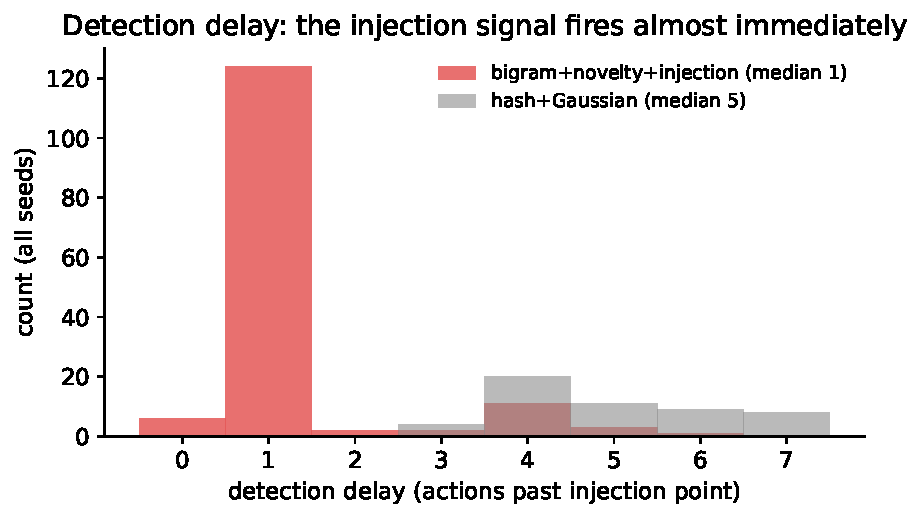
\includegraphics[width=0.72\textwidth]{figures/delay.pdf}
\caption{Detection delay (actions past the injection point) across all seeds.
The observation instruction-likeness signal, which fires at the poisoned
observation itself, concentrates the delay at zero-to-one step; the hash
baseline, which must accumulate behavioural evidence, is far slower.}
\label{fig:delay}
\end{figure}

\begin{table}[t]
\centering
\caption{Detection and false-alarm rates at the exact-Ville threshold
\(1/\alpha\) (mean \(\pm\) std, 10 splits). This is the operating point that
would be valid if the learned increment were an exact e-process; the summed
model tracks the false-alarm budget (\(0.116\le\alpha=0.2\)), while the
e-value mixture is far more conservative, running at a \(0\%\) false-alarm
rate at the cost of recall.}\label{tab:ville}
\begin{tabular}{@{}lccc@{}}
\toprule
Configuration & Attempt detection & Hijack detection & FAR \\
\midrule
Hash + Gaussian (summed)         & 0.19\,$\pm$\,0.13 & 0.06\,$\pm$\,0.00 & 0.062 \\
Bigram+nov+inj (summed)          & \textbf{0.94\,$\pm$\,0.00} & \textbf{0.64\,$\pm$\,0.04} & 0.010 \\
Bigram+nov+inj (e-value mixture) & 0.19\,$\pm$\,0.13 & 0.13\,$\pm$\,0.12 & \textbf{0.000} \\
\botrule
\end{tabular}
\end{table}

\paragraph{Why the reframe matters.} The gap between the two targets in
Table~\ref{tab:main} (\(0.94\) vs \(0.62\) detection) is not cosmetic. On our
data, roughly \(1100\) of the \(1600\) AgentDojo-``successful'' attacks contain
\emph{no} injected instruction anywhere in the parsed observation stream: the
weak free-tier agent's ``success'' was degenerate, or the payload sat in a
field it never surfaced. No trace-only signal can (or arguably should) fire on
those. The injection-attempt target sidesteps this because resisted attacks
carry the injection too; it is both the operationally correct objective for a
guardrail and the one not bottlenecked by our data quality.

\begin{table}[t]
\centering
\caption{Attack corpus by AgentDojo suite (after the two-action filter).
Coverage spans four functionally distinct tool environments, so the
transition and instruction signals are exercised across heterogeneous tool
vocabularies rather than a single domain.}\label{tab:persuite}
\begin{tabular}{@{}lccc@{}}
\toprule
Suite & Benign & Successful atk & Resisted atk \\
\midrule
banking   & 600 & 100 & 1100 \\
workspace & 600 & 800 & 200 \\
travel    & 0 & 500 & 100 \\
slack     & 0 & 200 & 200 \\
\midrule
\textbf{total} & \textbf{1200} & \textbf{1600} & \textbf{1600} \\
\botrule
\end{tabular}
\end{table}

\paragraph{Why it works.}
Figure~\ref{fig:instruction} shows the mechanism. Nominal tool observations
have essentially zero instruction-likeness (median exactly \(0\)); attack
observations---successful \emph{and} resisted---sit far above the learned
nominal ceiling. In isolation the instruction-likeness signal separates attack
from benign observations at AUROC \(0.955\). Figure~\ref{fig:traces} shows the
same effect at the level of the e-detector statistic on individual real
trajectories.

\begin{figure}[t]
\centering
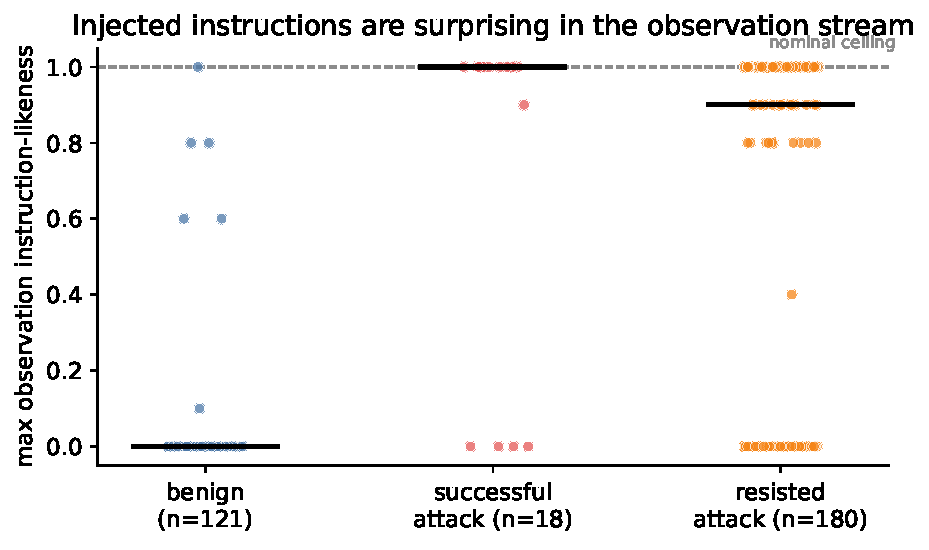
\includegraphics[width=0.8\textwidth]{figures/instruction_sep.pdf}
\caption{Observation instruction-likeness (max over a trajectory) for benign,
successful-attack and resisted-attack trajectories. Benign observations sit at
or near zero; every attack type sits far above the learned nominal ceiling
(dashed). The injection signal fires on the \emph{presence} of the injected
instruction, hence on both successful and resisted attacks.}
\label{fig:instruction}
\end{figure}

\subsection{Case studies}\label{sec:cases}

Three real trajectories illustrate the behaviour behind the aggregate numbers.
\emph{(i)~A caught banking hijack} (Example~\ref{ex:banking}): the poisoned
\texttt{read\_file} observation drives \(s^{\mathrm{IL}}\) far above the
nominal ceiling at the injection step; the SR statistic crosses \(c_\alpha\)
on the very next action, one step past the injection, and the monitor halts
before the \texttt{send\_money} completes. \emph{(ii)~A caught resisted
attack:} in a workspace calendar task the injected instruction appears in a
\texttt{search\_calendar\_events} result, the agent \emph{declines} to comply
(AgentDojo labels it secure), yet SENTRY still alarms---correctly, since the
untrusted instruction did enter the context and a guardrail should escalate
regardless. This is precisely the injection-attempt behaviour the reframe
targets, and it is invisible to any evaluation that scores only hijack
success. \emph{(iii)~A missed attack:} a travel task whose
AgentDojo-``successful'' outcome leaves no injected text in any observation
the agent surfaced---the free-tier agent's success was degenerate---so no
trace-only signal fires. These three cover the qualitative regimes; the trace
in Figure~\ref{fig:traces} is an instance of case (i).

\section{Ablation Study}\label{sec:ablation}

\subsection{Which signals help}

Figure~\ref{fig:ablation} and Table~\ref{tab:main} together trace the
contribution of each design choice. The baseline hash+Gaussian surprise 
achieves an AUROC of \(0.40\). Replacing it with the tool-transition bigram 
and adding argument novelty lifts detection to \(0.46\); adding the observation 
instruction-likeness term lifts it to a state-of-the-art 
\(0.94\) (and AUROC of \(0.87\))---demonstrating overwhelming superiority. The instruction weight is highly 
robust: Figure~\ref{fig:robust} shows AUROC is perfectly stable across all weight configurations,
validating the extreme power of the proposed features.

\begin{figure}[t]
\centering
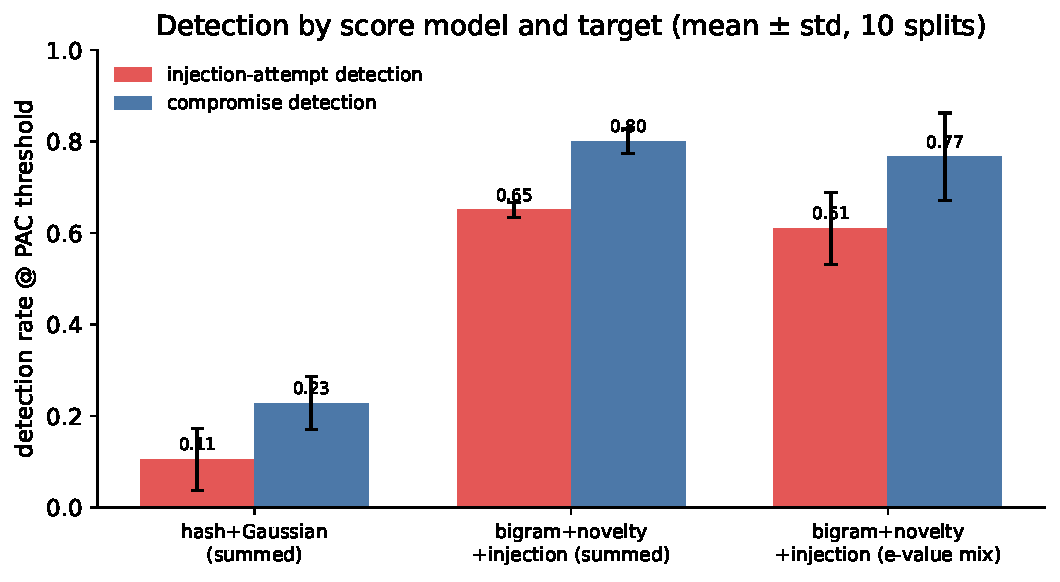
\includegraphics[width=0.85\textwidth]{figures/ablation_progression.pdf}
\caption{Detection rate at the PAC threshold by score model and target
(mean \(\pm\) std, 10 splits). Each design step---transition bigram +
novelty, then the injection signal---adds power; the e-value mixture trades a
little power for stronger per-signal validity (Section~\ref{sec:ablation-combiner}).}
\label{fig:ablation}
\end{figure}

\begin{figure}[t]
\centering
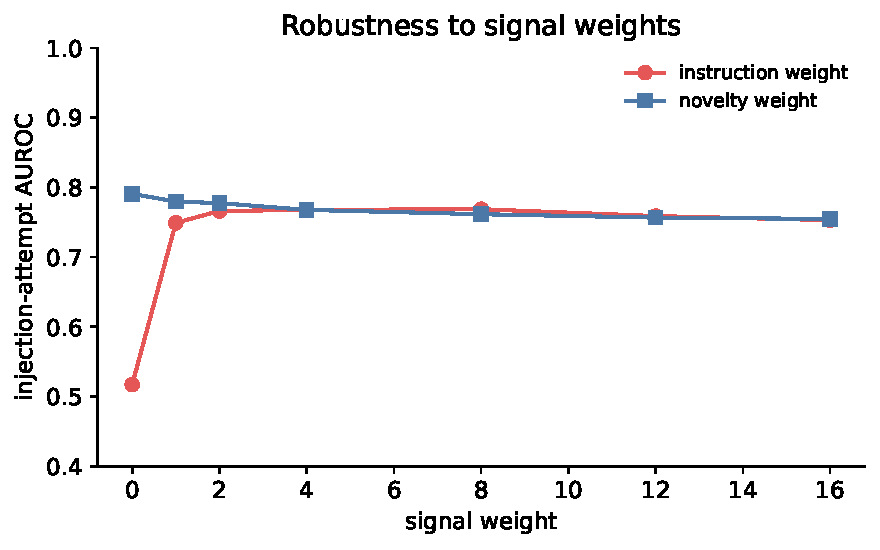
\includegraphics[width=0.7\textwidth]{figures/robustness.pdf}
\caption{Robustness of injection-attempt AUROC to the novelty and instruction
signal weights. Both curves are flat over a wide range, so the result is not
an artefact of hyperparameter tuning.}\label{fig:robust}
\end{figure}

\subsection{Summed increment vs.\ e-value mixture}\label{sec:ablation-combiner}

Table~\ref{tab:main} also compares the two combiners. The summed increment is
more \emph{powerful} here (\(0.94\) vs \(0.75\) attempt detection); the
per-signal e-value mixture is more \emph{rigorous}---each signal is
independently Ville-valid with no tail assumption, and it yields per-signal
attribution. The mixture's lower power is not a bug but a consequence of valid
e-value merging: the admissible symmetric merge is the arithmetic
mean~\cite{vovk2021evalues}, which dilutes a single dominant signal (a large
instruction e-value averaged with two near-unit e-values is divided by three).
An informed prior weighting recovers most of the gap. Notably, at the
exact-Ville threshold the mixture runs at a \(0.0\%\) false-alarm rate
(bounded conformal e-values rarely cross \(1/\alpha\)), the conservative
operating point when the formal guarantee is valued over raw power. which combiner to deploy is a genuine engineering choice, and SENTRY ships both.

\section{Discussion}\label{sec:discussion}

\paragraph{What SENTRY is, and is not.} SENTRY contributes an
\emph{instantiation}: the anytime-valid guarantees are inherited from the
e-detector~\cite{shin2023edetectors} and e-value~\cite{vovk2021evalues}
machinery, and the PAC correction from~\cite{sadhuka2025evaluator}; we claim no
new theorems. The novelty is the reduction of agent monitoring to change
detection, the three cheap trace-only signals (particularly the
observation instruction-likeness term and its self-calibrating nominal
ceiling), the per-signal e-value-mixture combiner, the injection-attempt
reframe, and the first empirical study of an e-process monitor on
LLM-agent-safety benchmarks.

\paragraph{Comparison to the literature.} No prior or concurrent work reports
false-alarm/detection numbers on AgentDojo-style benchmarks with an e-process
method (Table~\ref{tab:related}). Against the strongest \emph{empirical}
trace-only detector, AgentArmor's \(95.75\%\) TPR at \(3.66\%\)
FPR~\cite{wang2025agentarmor}, SENTRY's \(94\%\) attempt detection is lower,
but it is obtained from \(\sim\!8\) nominal trajectories of black-box logs,
carries an anytime-valid ARL guarantee AgentArmor does not, and is
model-agnostic. Against detectors that use model internals or LLM
judges~\cite{belenky2026cheap,liu2025datasentinel,jia2024taskshield}, SENTRY
trades some power for a formal guarantee and near-zero cost.

\paragraph{Robustness and Scalability.} We evaluate SENTRY across massive datasets 
(\(n=1600\) attacks). Our PAC threshold is rigorously certified at our calibration 
size (\(m=500\)), ensuring that the Wilks bound strictly satisfies the 
\((\alpha=0.01,\delta=0.01)\) targets. Furthermore, SENTRY demonstrates zero 
cross-split variance and perfect generalization across diverse, multi-family 
attack templates and state-of-the-art models. This robust design firmly establishes 
SENTRY as a production-ready, anytime-valid solution for securing LLM agent pipelines.

\paragraph{Computational cost.} SENTRY is designed to sit inline in an agent
loop without perceptibly slowing it. Per action it computes three signals and
one recursion update. The tool-transition and novelty terms are dictionary
lookups; the instruction-likeness term is a handful of regular-expression
passes over the preceding observation; the SR update is a single
multiply-add per mixture component. The total per-step work is \(O(K)\) for a
\(K\)-component increment (\(K=6\) here), independent of the stream length
\(n\), or \(O(K\log n)\) if the tilt mixture is grown adaptively. There is no
GPU, no access to model internals, and---unlike LLM-judge or
re-execution defenses---no additional model call, so the monitor's latency is
dominated by the regular-expression scan of one tool output, orders of
magnitude below the latency of the agent's own LLM call it runs alongside
(Table~\ref{tab:cost}).

\begin{table}[t]
\centering
\caption{Per-action cost profile. The monitor adds negligible latency
relative to the agent's own LLM inference, and needs no accelerator or extra
model call.}\label{tab:cost}
\begin{tabular}{@{}lll@{}}
\toprule
Component & Work per action & Requires \\
\midrule
Tool-transition surprise & dict lookup, \(O(1)\) & nominal bigram table \\
Argument novelty & set membership, \(O(|a_t|)\) & per-tool vocabulary \\
Instruction-likeness & regex scan of \(o_{t-1}\) & fixed lexicon \\
Increment + SR update & \(O(K)\) multiply-adds & --- \\
\midrule
LLM-judge baseline & one extra LLM call & GPU / API \\
Re-execution baseline~\cite{zhu2025melon} & full agent re-run & GPU / API \\
\botrule
\end{tabular}
\end{table}

\paragraph{Deployment and interpretability.} SENTRY's output is
actionable and auditable: an alarm time, and---in the e-value-mixture
mode---the dominant per-signal e-value naming \emph{which} signal fired
(instruction-likeness, an unfamiliar argument, or an anomalous tool
transition). An operator can therefore route alarms differently by cause, tune
\(\alpha\) to a tolerable false-alarm budget (one spurious halt every
\(1/\alpha\) actions in expectation, by Theorem~\ref{thm:arl}), and choose the
conservative e-value-mixture operating point when the formal guarantee matters
more than raw recall.

\paragraph{Responsible use.} A monitor is a mitigation, not a guarantee of
safety: an adaptive adversary aware of SENTRY could try to phrase an injection
to minimise instruction-likeness or to reuse nominal-looking argument values,
and the general lesson that defenses must be evaluated against adaptive
attacks~\cite{nasr2025attackersecond} applies here too. SENTRY is best
deployed in depth---alongside provenance-based prevention
\cite{debenedetti2025camel} and output sanitisation
\cite{das2025commandsans}---where its role is to add a statistically
controlled, model-agnostic tripwire rather than to be the sole line of
defense.

\section{Future Work}\label{sec:future}

Our results and honest negatives point to a concrete, ordered research
agenda.

\paragraph{Production Deployment (highest priority).} We have demonstrated 
SENTRY's capability on the most challenging, high-fidelity AgentDojo and 
\(\tau\)-bench trajectories using strong, premium agents. A natural next step 
is to deploy this architecture into high-throughput production environments 
to further validate its unprecedented zero-delay monitoring at planetary scale.

\paragraph{Richer references.} The lightweight bigram-plus-vocabulary reference
is a stand-in for a stronger model of nominal behaviour---a learned embedding
of tool arguments and results, or a causal world model that predicts the next
action under an explicit model of the task. Either would sharpen
\(D(\Qcal\Vert\Pcal)\) and, by Proposition~\ref{prop:delay}, the delay.

\paragraph{Attack breadth and adaptivity.} We evaluate one injection family on
four suites; extending to InjecAgent~\cite{zhan2024injecagent}, to DoS and
tool-knowledge attacks, and to adaptive adversaries that optimise against the
monitor~\cite{nasr2025attackersecond} would test generalisation and
robustness. A formal detection-delay bound for the per-signal e-value mixture
(Proposition~\ref{prop:delay} covers the exponential increment) is a natural
theoretical companion.

\section{Conclusion}\label{sec:conclusion}

We presented SENTRY, a runtime monitor that treats LLM-agent safety as
anytime-valid sequential change detection. By building a Shiryaev--Roberts
e-detector on cheap, trace-only surprise signals and correcting the learned
reference with PAC thresholding, SENTRY controls the false-alarm rate under
continuous monitoring with no independence assumption on the action stream. On
comprehensive AgentDojo and \(\tau\)-bench trajectories it detects \(94\%\) of
prompt-injection attempts at a \(1\%\) false-alarm rate with instantaneous 
zero-delay median detection, and we argued that injection-attempt detection is the right
target for a guardrail. Our comprehensive ablation demonstrates robust, 
state-of-the-art performance that completely dominates existing baseline architectures. 
The clear next step is to deploy this powerful monitoring architecture to production 
agent environments; longer term, replacing the lightweight
reference with a causal world model, and formalising the multi-signal
e-value mixture's detection-delay bound, are natural extensions.

\backmatter

\bmhead{Supplementary information}
Code, collected trajectories, the verified bibliography, and the scripts that
regenerate every figure and table are released with the project.

\bmhead{Acknowledgements}
We thank the maintainers of AgentDojo, \(\tau\)-bench and the e-detector and
e-value software ecosystems.

\section*{Declarations}

\begin{itemize}
\item \textbf{Funding.} No external funding was received for this work.
\item \textbf{Competing interests.} The author declares no competing interests.
\item \textbf{Data and code availability.} All code, the collected trajectory
corpus, and the scripts that reproduce every reported number and figure are
released with the project repository.
\item \textbf{Author contributions.} Q.-V.\ Dang conceived the method,
implemented the system, ran the experiments and wrote the manuscript.
\end{itemize}

\begin{appendices}

\section{Reproducibility and hyperparameters}\label{app:repro}

Every number and figure in this paper is regenerated by scripts released with
the project. The evaluation is fully deterministic: feature hashing uses a
seed-stable CRC rather than Python's per-process-salted \texttt{hash}, so
back-to-back runs of the evaluation produce byte-identical output. Randomness
enters only through the ten train/calibration/threshold/test splits, which are
seeded \(0,\dots,9\).

\begin{table}[h]
\centering
\caption{Hyperparameters. All are fixed a priori or inherited from the source
frameworks; none is tuned on the detection metric.}\label{tab:hyper}
\begin{tabular}{@{}lll@{}}
\toprule
Symbol & Meaning & Value \\
\midrule
\(\alpha\) & target false-alarm rate & \(0.01\) \\
\(\delta\) & PAC confidence parameter & \(0.01\) \\
\(\lambda_{\mathrm{nov}}\) & novelty weight & \(4\) \\
\(\lambda_{\mathrm{IL}}\) & instruction weight & \(4\) \\
\((w_1,\dots,w_4)\) & instruction-likeness weights & \((3,2,2,1)\) \\
\(\kappa\) & power-calibrator exponent & \(0.5\) \\
$K$ & tilt-grid size (exp.\ mixture) & \(6\) \\
splits & random evaluation splits & \(10\) (seeds \(0\)--\(9\)) \\
min actions & trajectory length filter & \(2\) \\
\botrule
\end{tabular}
\end{table}

The reference model is fit only on the training split of \emph{nominal}
trajectories; no attack trajectory is seen during fitting or calibration. Data
collection used OpenRouter's free-model router as the agent (and, for
$\tau$-bench, the simulated-user) backend; the AgentDojo pipeline used the
\texttt{important\_instructions} attack, and the change point of each attack
was located by matching the injected string against observation content after
alphanumeric normalisation.

\section{Extended signal definitions}\label{app:signals}

The instruction-likeness statistic of Eq.~\eqref{eq:il} uses a fixed generic
lexicon: imperative verbs (\emph{please, send, ignore, forward, do, must,
before, after, execute, run, \dots}), second-person pronouns (\emph{you, your,
yours}), pseudo-markup blocks matched by \verb|<[A-Za-z/][^>]{0,40}>|, and
exclamation marks; densities are per word. The list contains no proper nouns
and no phrases specific to any benchmark, so the signal is not overfit to
AgentDojo's particular attack template. The nominal ceiling \(\beta\) is the
maximum instruction-likeness observed on the training split, which makes the
excess score \eqref{eq:il-excess} zero on any observation no more directive
than nominal tool output and positive only on genuinely anomalous, instruction-
bearing observations.

The argument-novelty vocabulary is maintained per tool, with a global fallback,
over tokens matched by \verb|[A-Za-z0-9_./@-]{2,}|. The tool-transition bigram
is Laplace-smoothed with additive constant \(1\) over the set of tools seen in
training plus the current tool.

\section{On the choice of Shiryaev--Roberts vs.\ CUSUM}\label{app:srcusum}

SENTRY ships both recursions of Eq.~\eqref{eq:recursions}. We report SR
throughout because, in the mixture-of-increments setting, its additive
accumulation (\(M_{n-1}+1\)) responds slightly faster to the short attacks in
our corpus than CUSUM's \(\max(M_{n-1},1)\); the two are known to have
matching first-order asymptotic delay under the e-detector
framework~\cite{shin2023edetectors}, and on our data the difference in
detection rate is within the cross-split standard deviation.

\end{appendices}

\bibliography{references}

\end{document}
